\documentclass[11pt,a4paper,oneside]{report}
% Shared preamble. Everything here is stock TeX Live; no external downloads,
% so the manual builds on any machine that can build the workspace docs.
\usepackage[T1]{fontenc}
\usepackage[utf8]{inputenc}
\usepackage{lmodern}
\usepackage[a4paper,margin=25mm,headheight=14pt]{geometry}
\usepackage{microtype}

\usepackage{booktabs}
\usepackage{longtable}
\usepackage{array}
\usepackage{tabularx}
\usepackage{multirow}

\usepackage{graphicx}
\usepackage{tikz}
\usetikzlibrary{arrows.meta,positioning,shapes.geometric,fit,backgrounds,calc}
\usepackage{pgfplots}
\pgfplotsset{compat=1.18}

\usepackage{xcolor}
\usepackage{listings}
\usepackage{fancyhdr}
\usepackage{enumitem}
\usepackage[most]{tcolorbox}
\usepackage[hidelinks]{hyperref}

% ---------------------------------------------------------------- colours ---
\definecolor{codebg}{HTML}{F6F8FA}
\definecolor{coderule}{HTML}{D0D7DE}
\definecolor{keyword}{HTML}{0550AE}
\definecolor{comment}{HTML}{6E7781}
\definecolor{string}{HTML}{0A6E3B}
\definecolor{warnbg}{HTML}{FFF4E5}
\definecolor{warnrule}{HTML}{D97706}
\definecolor{notebg}{HTML}{EEF4FF}
\definecolor{noterule}{HTML}{3B6FD4}

% ----------------------------------------------------------------- code -----
\lstdefinestyle{shell}{
  basicstyle=\ttfamily\footnotesize,
  backgroundcolor=\color{codebg},
  frame=single, rulecolor=\color{coderule}, framesep=5pt,
  breaklines=true, breakatwhitespace=false,
  postbreak=\mbox{\textcolor{coderule}{$\hookrightarrow$}\space},
  columns=fullflexible, keepspaces=true,
  showstringspaces=false, upquote=true,
  literate={-}{{-}}1 {~}{{\textasciitilde}}1 {>}{{\textgreater}}1 {<}{{\textless}}1,
}
\lstdefinestyle{py}{style=shell,
  language=Python,
  keywordstyle=\color{keyword}\bfseries,
  commentstyle=\color{comment}\itshape,
  stringstyle=\color{string},
}
\lstset{style=shell}
\newcommand{\cmd}[1]{\texttt{\small #1}}

% --------------------------------------------------------------- callouts ---
% Support claims in this manual are bounded by dated gates. These two boxes are
% how that boundary stays visible instead of being buried in a paragraph.
\newtcolorbox{safetybox}[1][Safety]{
  breakable, enhanced, colback=warnbg, colframe=warnrule,
  boxrule=0.4pt, left=6pt, right=6pt, top=5pt, bottom=5pt,
  fonttitle=\bfseries\small, title={#1}}

\newtcolorbox{notebox}[1][Note]{
  breakable, enhanced, colback=notebg, colframe=noterule,
  boxrule=0.4pt, left=6pt, right=6pt, top=5pt, bottom=5pt,
  fonttitle=\bfseries\small, title={#1}}

% ---------------------------------------------------------------- headers ---
\pagestyle{fancy}
\fancyhf{}
\fancyhead[L]{\small\nouppercase{\leftmark}}
\fancyhead[R]{\small\thepage}
\renewcommand{\headrulewidth}{0.4pt}

\setlist{itemsep=2pt, parsep=0pt, topsep=4pt}
\setlength{\parskip}{4pt}
\setlength{\parindent}{0pt}

% --------------------------------------------------------------- graphics ---
% Screenshots need a GUI session, so they may legitimately be absent on a
% headless build. Missing artwork should not fail the build; it should be
% visibly missing. \graphicsorplaceholder{file}{width}{what it would show}
\newcommand{\graphicsorplaceholder}[3]{%
  \IfFileExists{#1}{\includegraphics[width=#2]{#1}}{%
    \fbox{\parbox[c][32mm][c]{#2}{\centering\small\itshape
      figure not generated\\[2pt]\footnotesize\normalfont #3\\[2pt]
      \texttt{\scriptsize bash docs/manual/figures/generate.sh}}}}%
}



\title{\Huge\bfseries Baxter on ROS 2 Jazzy\\[6pt]
  \large A workspace manual: simulation first, hardware under supervision}
\author{Yunus Danabas}
\date{Version 0.2.0 --- \today}

\begin{document}

\maketitle

\begin{abstract}
\noindent
This manual documents \texttt{baxter\_ros2\_jazzy}, a ROS~2 Jazzy workspace for the
Rethink Robotics Baxter Research Robot. It covers the simulation path
(Gazebo Harmonic, \texttt{ros2\_control}, MoveIt~2) end to end, and the hardware
path as far as dated, supervised gates have actually taken it.

Every hardware claim in this manual names the session that earned it. The
evidence base is one Baxter, driven under supervision, on four dated occasions.
That is a narrow base and the manual says so wherever it matters. Where something
was measured, the number is given; where something was not measured, it is listed
as not measured rather than assumed to work.
\end{abstract}

\tableofcontents

\chapter{Introduction}
\label{ch:intro}

\section{What this workspace is}

\texttt{baxter\_ros2\_jazzy} runs a Rethink Robotics Baxter Research Robot from
ROS~2 Jazzy. The default path is simulation: Gazebo Harmonic, \texttt{ros2\_control}
arm controllers, and MoveIt~2 planning against them. On top of that sits a
hardware path that talks to the robot's own ROS~1 Noetic master through a bridge,
and that path has moved a real arm --- under supervision, in dated sessions.

Baxter shipped in 2012 with a ROS~1 Groovy/Indigo SDK. Rethink Robotics closed in
2018 and there is no vendor ROS~2 support, so anything running Baxter on Jazzy is
reconstructing the command path from the robot's wire protocol outward. That is
what this workspace does, and it is why the hardware chapters read as carefully as
they do: nothing here is a supported vendor path.

\section{How to read the support claims}

Every capability statement in this manual falls into one of three categories, and
the manual is written so you can always tell which:

\begin{itemize}
  \item \textbf{Passed} --- a gate ran and its evidence is recorded. Simulation
    gates run in CI on every push.
  \item \textbf{Passed, supervised} --- it worked on one physical robot, on a named
    date, with a person holding the e-stop. This is not general support.
  \item \textbf{Deferred} or \textbf{not measured} --- said plainly rather than
    left to inference.
\end{itemize}

\begin{safetybox}[The evidence base, stated once]
Every hardware claim in this manual comes from \emph{one} Baxter, driven under
supervision, on four dated occasions: 2026-07-22 (bridge and interlocks),
2026-07-24 (first supervised motion, first MoveIt execution), and 2026-07-25
(speed characterisation and a MoveIt re-run). Sustained duty, gripper commands,
and any second robot are unmeasured. Do not read this manual as evidence that
Baxter is generally supported on ROS~2.
\end{safetybox}

The canonical machine-readable version of this is
\texttt{docs/support\_matrix.md} in the repository; if that file and this manual
ever disagree, the file wins, because CI checks it and nothing checks prose.

\section{What works}

\begin{table}[h]
\centering
\small
\begin{tabularx}{\linewidth}{@{}lllX@{}}
\toprule
\textbf{Profile} & \textbf{Status} & \textbf{Chapter} & \textbf{Notes} \\
\midrule
Gazebo sim & passed & \ref{ch:sim} & Both arms, 17 joint states, reversible motion. \\
Gazebo + RViz & passed & \ref{ch:sim} & RobotModel/TF profile. \\
MoveIt~2 sim & passed & \ref{ch:moveit} & OMPL, single- and dual-arm groups. \\
MoveIt RViz & passed & \ref{ch:moveit} & MotionPlanning panel, IK markers. \\
Hardware bridge & supervised & \ref{ch:bridge} & 2026-07-22. \\
Supervised motion & supervised & \ref{ch:hwmotion} & 2026-07-24; speed limits 2026-07-25. \\
MoveIt on hardware & supervised, \emph{limited} & \ref{ch:hwmotion} & Left arm aborts most goals at default speed. \\
Grippers, cameras, Zenoh & deferred & --- & No gate requires them yet. \\
\bottomrule
\end{tabularx}
\end{table}

\section{What this manual will not tell you}

It does not contain raw safety-topic publishing or hardware enable commands.
Those exist in the repository's operational runbook, behind procedures that
assume a supervised session and an e-stop within reach. A manual that teaches
someone to energise a 2-metre dual-arm robot from a code snippet is a manual that
has misjudged its audience.

It also does not document the Rethink Intera manufacturing workflow --- task
training, vacuum grippers, Modbus, the factory pick-and-place tooling. That is a
different product built on the same hardware. If you have a manufacturing Baxter
and want to train pick-and-place tasks by demonstration, this workspace is not
what you want.

\section{Layout}

Chapter~\ref{ch:platform} covers the robot itself: joints, limits, and the
concepts the rest of the manual assumes. Chapters~\ref{ch:install}
to~\ref{ch:moveit} are the simulation path, which needs no robot and is where
anyone should start. Chapters~\ref{ch:bridge} and~\ref{ch:hwmotion} are the
hardware path. Chapter~\ref{ch:verify} is how to check that a change did not break
anything, without a robot. The appendices are the condensed command sheet and the
numeric tables.

\chapter{The Baxter platform}
\label{ch:platform}

This chapter is background: what the hardware is, what its joints are called, and
which of the legacy ROS~1 concepts survive into this workspace. Everything here
is factual description of the robot, drawn from the Rethink documentation set and
from what the robot was observed to do during the hardware sessions.

\section{The robot}

Baxter is a two-armed research robot on a fixed pedestal. Each arm has seven
revolute joints; the arms are series-elastic, so every joint has a spring between
the motor and the link. That single design choice explains most of what
Chapter~\ref{ch:hwmotion} measures: the arm is compliant by construction, it does
not track a fast setpoint rigidly, and lag is a physical property rather than a
tuning defect.

The workspace also carries a head with a pan joint, a screen, and two
one-degree-of-freedom electric grippers. This workspace commands the arms only.
The head pan and the two gripper finger joints are published as state and are not
commanded; the model provides them so that TF and the robot display are complete.

\section{Joint naming}

Joints are named \texttt{<side>\_<segment>}, where side is \texttt{left} or
\texttt{right}. The seven suffixes, in chain order from the torso outward:

\begin{center}
\resizebox{\linewidth}{!}{% The seven arm joints in chain order, with the URDF limits the shim enforces.
% Values from follow_joint_trajectory_shim.py JOINT_LIMITS, transcribed from
% baxter_description/urdf/baxter_base/baxter_base.urdf.xacro.
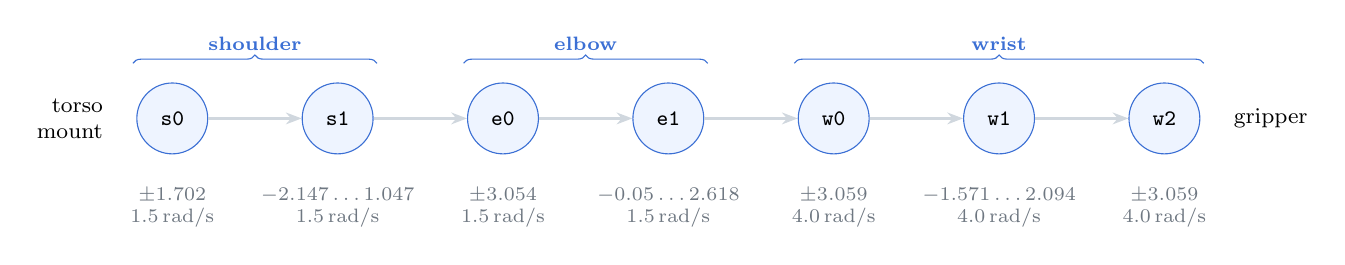
\begin{tikzpicture}[
  font=\small,
  j/.style={draw, circle, minimum size=9mm, inner sep=0pt, fill=notebg,
            draw=noterule, font=\footnotesize\ttfamily},
  seg/.style={-{Stealth[length=2mm]}, thick, draw=coderule},
  lim/.style={font=\scriptsize, align=center, text=comment},
  grp/.style={font=\scriptsize\bfseries, text=noterule},
]

\node[j] (s0) at (0,0) {s0};
\node[j] (s1) at (2.1,0) {s1};
\node[j] (e0) at (4.2,0) {e0};
\node[j] (e1) at (6.3,0) {e1};
\node[j] (w0) at (8.4,0) {w0};
\node[j] (w1) at (10.5,0) {w1};
\node[j] (w2) at (12.6,0) {w2};

\foreach \a/\b in {s0/s1, s1/e0, e0/e1, e1/w0, w0/w1, w1/w2}
  \draw[seg] (\a) -- (\b);

\node[left=3mm of s0, align=right, font=\footnotesize] {torso\\mount};
\node[right=3mm of w2, align=left, font=\footnotesize] {gripper};

\node[lim, below=3mm of s0] {$\pm 1.702$\\1.5\,rad/s};
\node[lim, below=3mm of s1] {$-2.147 \ldots 1.047$\\1.5\,rad/s};
\node[lim, below=3mm of e0] {$\pm 3.054$\\1.5\,rad/s};
\node[lim, below=3mm of e1] {$-0.05 \ldots 2.618$\\1.5\,rad/s};
\node[lim, below=3mm of w0] {$\pm 3.059$\\4.0\,rad/s};
\node[lim, below=3mm of w1] {$-1.571 \ldots 2.094$\\4.0\,rad/s};
\node[lim, below=3mm of w2] {$\pm 3.059$\\4.0\,rad/s};

\node[grp] at (1.05,0.95) {shoulder};
\node[grp] at (5.25,0.95) {elbow};
\node[grp] at (10.5,0.95) {wrist};

\draw[decorate, decoration={brace, amplitude=3pt}, draw=noterule]
  (-0.5,0.7) -- (2.6,0.7);
\draw[decorate, decoration={brace, amplitude=3pt}, draw=noterule]
  (3.7,0.7) -- (6.8,0.7);
\draw[decorate, decoration={brace, amplitude=3pt}, draw=noterule]
  (7.9,0.7) -- (13.1,0.7);

\end{tikzpicture}
}
\end{center}

\begin{itemize}
  \item \texttt{s0}, \texttt{s1} --- shoulder rotation and flexion.
  \item \texttt{e0}, \texttt{e1} --- upper-arm roll and elbow flexion.
  \item \texttt{w0}, \texttt{w1}, \texttt{w2} --- wrist roll, flexion, and final roll.
\end{itemize}

Two features of that table matter later. First, \texttt{s1} is the only strongly
asymmetric joint ($-2.147$ to $1.047$\,rad): a move that fits in one direction may
not fit in the other, which is why the example clients pick a reversible target
rather than a fixed offset. Second, the three wrist joints permit
$4.0$\,rad/s against $1.5$\,rad/s for the shoulder and elbow --- so a planner that
distributes motion evenly across joints will drive the wrists fastest. That is
the mechanism behind the MoveIt hardware limitation in
Section~\ref{sec:moveit-hardware}.

\section{Tucked and untucked}

Baxter parks with its arms folded against the torso. In that pose \texttt{s1}
sits at approximately $-2.175$\,rad, which is \emph{outside} the URDF limit table
this workspace enforces ($-2.147$). This is not a transcription error: the parked
pose is a mechanical rest position rather than a commanded one.

The consequence is deliberate and worth stating early. This workspace's action
shim rejects any goal containing an out-of-limit position, so while the robot is
tucked it will refuse to move --- correctly. Untucking is therefore done with the
legacy Rethink tool, not through the ROS~2 path, and Chapter~\ref{ch:bridge}
explains why replacing that tool is the one part of the legacy stack this project
does not simply reimplement.

\section{Enabling}

Baxter's arms are unpowered until the robot is explicitly enabled, and it reports
its state on \texttt{/robot/state} as an \texttt{AssemblyState}: enabled, stopped,
in error, and whether an estop is engaged. Motion requires enabled, not stopped,
no error.

An enable can be refused. If the robot believes its arms are in collision --- which
the tucked pose can trigger --- the enable is dropped almost immediately.
The legacy untuck tool works around this by suppressing collision avoidance on
both limbs at 20\,Hz \emph{while} it republishes the enable, rather than enabling
once and waiting. That detail is not a curiosity: it is the difference between an
enable that holds and one that does not, and it was rediscovered the hard way
during the 2026-07-22 session.

\begin{safetybox}
An enabled Baxter has powered arms. In gravity-compensation mode --- enabled but
uncommanded --- the arms hold position but move freely if pushed, and they will
drift. Never enable the robot without the e-stop in reach and the workspace clear.
\end{safetybox}

\section{The legacy ROS 1 interface}

The robot runs its own ROS~1 Noetic master. Everything this workspace does on
hardware is a client of that master. The topics that matter:

\begin{table}[h]
\centering
\small
\begin{tabularx}{\linewidth}{@{}llX@{}}
\toprule
\textbf{Topic} & \textbf{Type} & \textbf{Role} \\
\midrule
\texttt{/robot/state} & \texttt{AssemblyState} & Enabled, stopped, error, estop. The safety gate reads this. \\
\texttt{/robot/joint\_states} & \texttt{JointState} & Measured positions. Published by more than one node. \\
\texttt{/robot/ref\_joint\_states} & \texttt{JointState} & The robot's own commanded reference, $\approx$140\,Hz. \\
\texttt{/robot/limb/*/joint\_command} & \texttt{JointCommand} & Position commands in. \\
\texttt{robot/set\_super\_enable} & \texttt{Bool} & Enable/disable. \\
\bottomrule
\end{tabularx}
\end{table}

\begin{notebox}[One measurement worth carrying forward]
\texttt{/robot/joint\_states} is published by \emph{two} nodes --- arm joints from
one, gripper joints from another. A subscriber that keeps only the latest message
therefore sees an incomplete picture roughly a third of the time. Any client that
reads joint positions on hardware has to merge across messages by name. This is
handled in the workspace's clients and is called out again in
Section~\ref{sec:jointstate-merge}, because it is the kind of defect that looks
like flaky hardware.
\end{notebox}

Commanded motion is not fire-and-forget. \texttt{JointCommand} has a timeout: if
commands stop arriving for longer than \texttt{joint\_command\_timeout}
(0.2\,s by default), the arm reverts to gravity compensation. Holding a position
means continuing to command it, which is why the shim in
Chapter~\ref{ch:bridge} publishes at 100\,Hz for as long as a goal is active and
keeps commanding the final point after the trajectory ends.

\chapter{Installation}
\label{ch:install}

Nothing in this chapter needs a robot. The result is a workspace that runs the
full simulation path.

\section{Prerequisites}

Ubuntu 24.04 Noble with ROS~2 Jazzy. The tested profile is exactly that
combination; nothing else has passed a gate.

\begin{lstlisting}
sudo apt install -y \
  ros-jazzy-desktop ros-jazzy-ros-gz ros-jazzy-gz-ros2-control \
  ros-jazzy-ros2-control ros-jazzy-ros2-controllers \
  ros-jazzy-moveit ros-jazzy-robot-state-publisher ros-jazzy-xacro \
  ros-jazzy-joint-state-publisher-gui \
  python3-colcon-common-extensions python3-rosdep python3-vcstool
\end{lstlisting}

\section{Source and the dependency pin}

One external repository is imported, at a full commit SHA:

\begin{lstlisting}
git clone https://github.com/yunusdanabas/baxter_ros2_jazzy.git
cd baxter_ros2_jazzy
source /opt/ros/jazzy/setup.bash
mkdir -p src
vcs import src < repos/baxter_core.repos
git -C src/baxter_common_ros2 rev-parse HEAD
# expect: 678bfabea8c895b4134951a6c076217a90b9e0e6
\end{lstlisting}

That import brings the CentraleNantes \texttt{baxter\_common\_ros2} message and
description packages. The pin is a full SHA rather than a branch on purpose: the
robot description and message definitions determine wire compatibility with a
physical robot, and a branch that moves underneath a hardware session is a defect
waiting for the worst possible moment.

If \texttt{src/baxter\_common\_ros2} already exists, verify the SHA rather than
re-importing over local changes.

\section{Build}

\begin{lstlisting}
rosdep install --from-paths src --ignore-src -r -y
colcon build --base-paths src --symlink-install --packages-skip baxter_bridge
source install/setup.bash
\end{lstlisting}

\texttt{--packages-skip baxter\_bridge} is not optional. That package links ROS~1
libraries which do not exist on a clean Jazzy machine; it belongs on a bridge host
with both distributions installed, and this workspace does not use it --- the
hardware path uses a pure-Python bridge instead (Chapter~\ref{ch:bridge}).

If the workspace or its underlay changes, remove \texttt{build/}, \texttt{install/}
and \texttt{log/} before rebuilding, and never hand-edit generated setup files.

\begin{safetybox}[The conda trap, which does not announce itself]
If a conda or mamba environment is active, its \texttt{python3} comes first on
\texttt{PATH}. \texttt{setuptools} bakes the active interpreter into the shebang
of every installed console script at \emph{build} time, so the build succeeds and
then every \texttt{ros2 run} fails at runtime with
\texttt{No module named 'rclpy.\_rclpy\_pybind11'}, because \texttt{rclpy}'s C
extension is built against the system interpreter.

Check before building, not after:

\begin{lstlisting}
conda deactivate
which python3      # want /usr/bin/python3
\end{lstlisting}

A successful build is not evidence that this is fine.
\end{safetybox}

\section{Verify}

\begin{lstlisting}
bash scripts/sim_smoke.sh gates
\end{lstlisting}

This runs the hardware-free checks: compile, lint, unit tests, the 25-case
hardware-bridge dry run, URDF expansion, and the MoveIt collision-matrix check.
It needs no Gazebo and no GPU. Chapter~\ref{ch:verify} describes what each check
is actually protecting.

\chapter{Simulation}
\label{ch:sim}

\section{Launching}

\begin{lstlisting}
# headless server, the default for scripted checks
ros2 launch baxter_gz_sim sim.launch.py headless:=true

# with the Gazebo GUI
ros2 launch baxter_gz_sim sim.launch.py headless:=false

# with RViz as well
ros2 launch baxter_gz_sim sim_rviz.launch.py headless:=false
\end{lstlisting}

Run one simulation at a time.

\begin{notebox}[Do not reach for \texttt{ROS\_DOMAIN\_ID}]
It is tempting to isolate concurrent runs with a domain ID or a Gazebo partition.
Do not. The documented workflow runs a single simulation, and setting a domain has
silently split the bridge from the action shim --- two halves of one system, each
convinced the other was absent. If you need isolation, stop the other simulation.
\end{notebox}

\section{The model}

The simulation URDF fixes \texttt{world}~$\rightarrow$~\texttt{base} at
$z=0.92418$\,m, which puts the bottom of the pedestal on the floor. This is a
fixed joint, not a floating base with a settle phase: the robot is bolted down in
reality and a drop-and-settle would only add nondeterminism to every test that
follows. Both arms start at the SRDF neutral state.

\begin{figure}[h]
\centering
\graphicsorplaceholder{figures/sim_rviz.png}{\linewidth}{the plain RViz profile
with the RobotModel and TF displays}
\caption{\texttt{sim\_rviz.launch.py}. Fixed frame \texttt{world}, Global Status
Ok, RobotModel and TF displays active. This is the profile to check first: if the
model does not appear here, nothing in Chapter~\ref{ch:moveit} will work either.}
\label{fig:simrviz}
\end{figure}

\begin{figure}[h]
\centering
\graphicsorplaceholder{figures/tf_tree.pdf}{\linewidth}{the kinematic tree
derived from the simulation URDF}
\caption{Kinematic tree from \texttt{baxter\_gz\_control.urdf.xacro}. Dashed
edges are fixed joints; the arm joints are the seven per side that carry position
commands.}
\label{fig:tftree}
\end{figure}

Seventeen joints publish state: fourteen arm joints, \texttt{head\_pan}, and one
finger joint per gripper. Fourteen accept position commands --- the arms only.

\section{Controllers}

\begin{table}[h]
\centering
\small
\begin{tabularx}{\linewidth}{@{}lX@{}}
\toprule
\textbf{Controller} & \textbf{Interface} \\
\midrule
\texttt{left\_arm\_controller} & \texttt{/left\_arm\_controller/follow\_joint\_trajectory} \\
\texttt{right\_arm\_controller} & \texttt{/right\_arm\_controller/follow\_joint\_trajectory} \\
\texttt{joint\_state\_broadcaster} & publishes \texttt{/joint\_states} \\
\bottomrule
\end{tabularx}
\end{table}

\begin{lstlisting}
ros2 control list_controllers      # all three must be active
ros2 topic echo /joint_states --once
\end{lstlisting}

Command limits are enforced at the controller manager
(\texttt{enforce\_command\_limits: true}), and every arm joint carries a
trajectory and goal constraint. The goal constraint is $0.02$\,rad, which is the
number every example client checks itself against.

\section{The smoke client}

\begin{lstlisting}
ros2 launch baxter_examples sim_tiny_trajectory.launch.py
\end{lstlisting}

For each arm in turn the client reads a fresh joint state, picks a limit-safe
reversible target, commands it, verifies the final position against a fresh
reading, and returns to the measured start. Action success alone is not treated
as a pass: the client re-reads the state and compares. An action server that
reports success while the arm did not move is exactly the failure worth catching.

Useful parameters:

\begin{table}[h]
\centering
\small
\begin{tabularx}{\linewidth}{@{}llX@{}}
\toprule
\textbf{Parameter} & \textbf{Default} & \textbf{Effect} \\
\midrule
\texttt{joint} & \texttt{s1} & Which joint moves. Any of \texttt{s0 s1 e0 e1 w0 w1 w2}. \\
\texttt{offset} & 0.35\,rad & How far. \\
\texttt{duration} & 3.0\,s & How long, so offset/duration sets speed. \\
\texttt{cancel\_after\_sec} & 0.0 & Cancel mid-motion and verify the hold. \\
\bottomrule
\end{tabularx}
\end{table}

Both arms always move the same joint. That is the point of the parameter: on
hardware, comparing the same joint left against right is what distinguishes an
asymmetric \emph{plan} from an asymmetric \emph{arm}
(Section~\ref{sec:moveit-hardware}).

\section{Cancellation}

\begin{lstlisting}
ros2 run baxter_examples sim_tiny_trajectory --ros-args \
    -p use_sim_time:=true -p cancel_after_sec:=1.0
\end{lstlisting}

The requirement is not merely that cancellation is accepted. The arm must
\emph{hold} where it stopped, not sag, and the client verifies that by measuring
drift after the cancel. A cancel that drops the arm into gravity compensation
would pass a naive check and is a safety-relevant difference on hardware.

\section{Expected diagnostics}

Some Gazebo complaints are normal and should not be chased:

\begin{table}[h]
\centering
\small
\begin{tabularx}{\linewidth}{@{}lX@{}}
\toprule
\textbf{Message} & \textbf{Why it is expected} \\
\midrule
DART cannot create the gripper mimic constraint & Arm-only scope. Gripper TF is available; contact fidelity is not claimed. \\
Controller period 100\,Hz slower than physics at 1\,kHz & Controllers need not run every physics step. \\
Executor unavailable during hardware initialization & Benign if successful initialisation follows immediately. \\
Gazebo exits $-2$ after one Ctrl+C & Normal SIGINT status. \\
\bottomrule
\end{tabularx}
\end{table}

Missing joints, disabled command limits, controller failure, TF gaps, hangs, and
leftover processes are \emph{not} in this category.

\section{Scope}

Only arm joints are controlled. Grippers, cameras, obstacle sensing, and
compatibility fallbacks are outside this profile. Headless Gazebo is camera-less
by construction, so any camera work needs a dedicated path that does not exist
yet.

\chapter{MoveIt 2}
\label{ch:moveit}

\section{Launching}

\begin{lstlisting}
# move_group against the simulated controllers
ros2 launch baxter_moveit_config sim_moveit.launch.py headless:=true

# and the MotionPlanning RViz panel
ros2 launch baxter_moveit_config sim_moveit_rviz.launch.py headless:=false
\end{lstlisting}

Wait for \texttt{You can start planning now!} and a log line naming pipeline
\texttt{ompl}. The launch is readiness-gated: it waits for the simulation to be
up before starting \texttt{move\_group}, because a \texttt{move\_group} that
loads before the controllers exist comes up without them and then fails to
execute anything it plans.

\begin{figure}[h]
\centering
\graphicsorplaceholder{figures/moveit_rviz.png}{0.92\linewidth}{the RViz
MotionPlanning panel with the \texttt{both\_arms} group selected}
\caption{The MotionPlanning panel loaded correctly: a populated planning group,
Global Status Ok, and a 6-DOF interactive marker on each gripper. Note the
Velocity Scaling of 0.30 --- that is the RViz default and is fine in simulation.
On hardware it is too fast; see Section~\ref{sec:moveit-hardware}.}
\label{fig:moveitrviz}
\end{figure}

\section{Groups}

Five groups are defined: \texttt{left\_arm}, \texttt{right\_arm},
\texttt{both\_arms}, and a hand group per side. Named states
\texttt{left\_neutral} and \texttt{right\_neutral} match the simulation's initial
joint values exactly --- CI asserts that equality, because a neutral pose that
drifts from the model's start state makes every "return to neutral" a silent
small motion.

Planning uses OMPL with \texttt{RRTConnectkConfigDefault} as the default for all
three arm groups.

\section{The example clients}

\begin{lstlisting}
ros2 run baxter_examples moveit_left_tiny
ros2 run baxter_examples moveit_tiny --ros-args -p group:=right_arm
ros2 run baxter_examples moveit_tiny --ros-args -p group:=both_arms
\end{lstlisting}

Same contract as the direct client: fresh state, bounded reversible target,
verified against a fresh reading, returned to start. Add
\texttt{-p cancel\_after\_sec:=1.0} to exercise cancellation.

\begin{notebox}[These clients refuse to touch hardware]
\texttt{moveit\_left\_tiny} checks that \texttt{/move\_group} is running on
simulated time and refuses to send a goal otherwise. It is deliberate: a sim
example that could be pointed at a real robot by changing one launch file is a
sim example waiting to move an arm nobody was watching. Hardware MoveIt execution
is driven from the RViz panel by a person, as described in
Section~\ref{sec:moveit-hardware}.
\end{notebox}

\section{Cartesian goals and IK}

\begin{lstlisting}
# absolute point
ros2 run baxter_examples moveit_pose --ros-args \
    -p group:=left_arm -p x:=0.55 -p y:=0.25 -p z:=0.15

# relative nudge
ros2 run baxter_examples moveit_pose --ros-args \
    -p group:=left_arm -p delta_z:=0.05

# plan only, do not execute
ros2 run baxter_examples moveit_pose --ros-args \
    -p group:=left_arm -p delta_z:=0.05 -p plan_only:=true
\end{lstlisting}

Targets are position-only against a 3\,cm tolerance sphere in \texttt{torso} by
default, so gripper orientation is whatever IK picks. Absolute and relative forms
are mutually exclusive. \texttt{plan\_only} is the form to use first whenever
\texttt{move\_group} is attached to anything that can move.

For pure IK queries without motion:

\begin{lstlisting}
ros2 run baxter_examples ik_service_client --ros-args -p limb:=left
ros2 run baxter_examples ik_service_client --ros-args -p limb:=left -p x:=9.0
\end{lstlisting}

The second is deliberately unreachable and must exit non-zero with
\texttt{INVALID POSE}. A solver that never reports failure is not a solver, and
the verification script asserts that failure explicitly.

\section{The collision matrix}

\texttt{config/baxter.srdf} carries exactly 54 \texttt{disable\_collisions} pairs.
That is sparse for a robot this size, and two of those pairs were added by hand:

\begin{center}
\texttt{left\_upper\_elbow} $\leftrightarrow$ \texttt{left\_upper\_shoulder}\\
\texttt{right\_upper\_elbow} $\leftrightarrow$ \texttt{right\_upper\_shoulder}
\end{center}

Those links are two apart in the chain and graze by about 1.7\,mm in the pose the
untuck tool leaves the robot in. Without the pairs disabled, \texttt{move\_group}
returns $-10$ \texttt{START\_STATE\_IN\_COLLISION} and refuses to plan from the
robot's own resting pose.

The MoveIt Setup Assistant cannot rediscover them. Its sampling does not converge
for this model --- runs from ten thousand to two million trials produced matrices
between 263 and 311 pairs that disabled head, gripper and screen pairs that should
not be disabled, while still missing these two. So a regenerated matrix is a
regression, and the checked-in one stays.

\begin{safetybox}[If you regenerate the SRDF]
Run \texttt{scripts/check\_srdf.py diff OLD NEW} before and after. CI asserts
both pairs are present and that the total is exactly 54; the check exists because
this failure only shows up on hardware, at the moment you most want to plan.
\end{safetybox}

\chapter{The hardware bridge}
\label{ch:bridge}

\begin{safetybox}[Read this before the rest of the chapter]
Everything from here on can move a two-metre dual-arm robot. The operational
procedure --- network setup, sonar, enable, untuck, abort --- lives in the
repository's hardware runbook and command sheet, and assumes a supervised session
with the e-stop in hand. This chapter explains how the software works and why;
it is not a substitute for the runbook.
\end{safetybox}

\section{Shape of the problem}

Baxter runs a ROS~1 Noetic master. ROS~2 Jazzy cannot talk to it. The conventional
answer is \texttt{ros1\_bridge} on a host with both distributions installed, which
means maintaining a Noetic environment on Ubuntu 24.04 --- a container, in
practice, and a five-gigabyte one.

This workspace takes a different route. \texttt{scripts/py\_bridge.py} is a
pure-Python ROS~1 client: XML-RPC to the master, raw TCPROS to peers, no
\texttt{rospy} and no ROS~1 installation anywhere. It runs on the same laptop as
the ROS~2 side.

\begin{figure}[h]
\centering
\resizebox{\linewidth}{!}{% Hardware command path: ROS 1 master on the robot, through the pure-Python
% bridge, to the ROS 2 side. Drawn from scripts/py_bridge.py and
% src/baxter_hardware_bridge/.
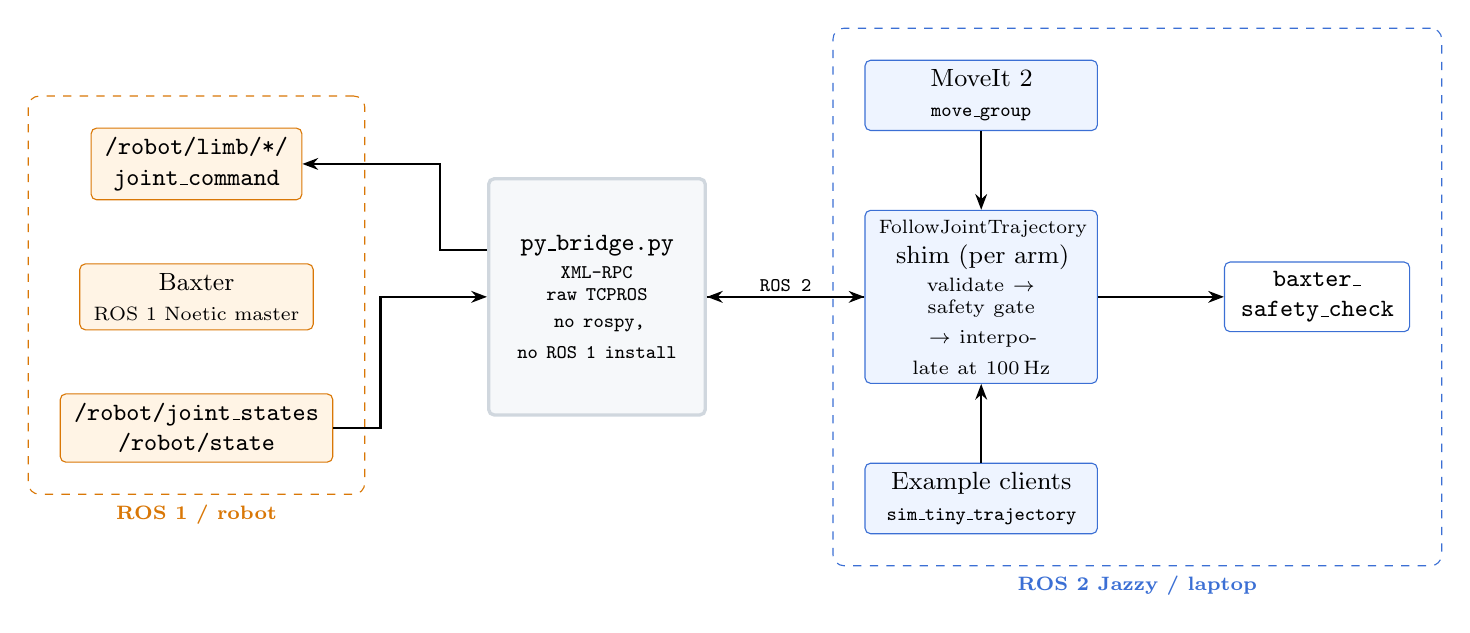
\begin{tikzpicture}[
  font=\small,
  node distance=6mm,
  box/.style={draw, rounded corners=2pt, align=center, minimum height=8mm,
              inner xsep=5pt, fill=white},
  ros1/.style={box, fill=warnbg, draw=warnrule},
  ros2/.style={box, fill=notebg, draw=noterule},
  bridge/.style={box, fill=codebg, draw=coderule, very thick},
  flow/.style={-{Stealth[length=2mm]}, thick},
  lbl/.style={font=\scriptsize\ttfamily, inner sep=1.5pt, fill=white},
]

\node[ros1] (robot)  {Baxter\\\scriptsize ROS~1 Noetic master};
\node[ros1, below=8mm of robot] (jointstates) {\ttfamily/robot/joint\_states\\\ttfamily/robot/state};
\node[ros1, above=8mm of robot] (jointcmd) {\ttfamily/robot/limb/*/\\\ttfamily joint\_command};

\node[bridge, right=22mm of robot, minimum height=30mm, text width=24mm]
  (bridge) {\ttfamily py\_bridge.py\\[2pt]\scriptsize XML-RPC\\\scriptsize raw TCPROS\\[2pt]\scriptsize no rospy,\\\scriptsize no ROS~1 install};

\node[ros2, right=20mm of bridge, text width=26mm] (shim)
  {\scriptsize FollowJointTrajectory\\\small shim (per arm)\\[2pt]\scriptsize validate $\rightarrow$ safety gate\\\scriptsize $\rightarrow$ interpolate at 100\,Hz};

\node[ros2, above=10mm of shim, text width=26mm] (moveit) {MoveIt~2\\\scriptsize\ttfamily move\_group};
\node[ros2, below=10mm of shim, text width=26mm] (clients) {Example clients\\\scriptsize\ttfamily sim\_tiny\_trajectory};

\node[box, right=16mm of shim, draw=noterule, text width=20mm] (safety)
  {\ttfamily baxter\_\\safety\_check};

\draw[flow] (jointstates.east) -- ++(6mm,0) |- (bridge.west);
\draw[flow] (bridge.west) ++(0,6mm) -- ++(-6mm,0) |- (jointcmd.east);
\draw[flow] (bridge) -- node[lbl,above]{ROS~2} (shim);
\draw[flow] (shim) -- (bridge);
\draw[flow] (moveit) -- (shim);
\draw[flow] (clients) -- (shim);
\draw[flow] (shim) -- (safety);

\begin{scope}[on background layer]
  \node[draw=warnrule, dashed, rounded corners, inner sep=4mm,
        fit=(jointcmd)(robot)(jointstates), label={[font=\scriptsize\bfseries,
        text=warnrule]below:ROS 1 / robot}] {};
  \node[draw=noterule, dashed, rounded corners, inner sep=4mm,
        fit=(moveit)(shim)(clients)(safety), label={[font=\scriptsize\bfseries,
        text=noterule]below:ROS 2 Jazzy / laptop}] {};
\end{scope}

\end{tikzpicture}
}
\caption{The hardware command path. The bridge is a ROS~1 protocol client, not a
ROS~1 installation; the shim is where every safety decision is made.}
\label{fig:arch}
\end{figure}

\subsection{Why this is smaller than it sounds}

Subscribing to a ROS~1 topic requires negotiating a TCPROS connection, and the
handshake includes an MD5 sum of the message definition. The bridge answers
\texttt{"md5sum": "*"} --- a wildcard --- on the subscribe side. The master accepts
it, so \emph{receiving} a new message type needs no MD5 table and no message
definition, only code that can interpret the payload bytes. That is why adding a
topic is usually a dozen lines.

Publishing is not symmetric. \texttt{rosbag} records whatever the publisher
advertised, so a wildcard MD5 produced recordings that could not be deserialised
afterwards --- our own data, unreadable. The publisher side now answers with the
real MD5 and message definition for the types it publishes. Unlisted types still
fall back to the wildcard and still work on the wire; they just do not record
usefully.

\section{The action shim}

\texttt{FollowJointTrajectory} is what MoveIt and the example clients speak. The
robot does not: it accepts position commands on \texttt{joint\_command} and
expects them to keep arriving. The shim bridges that gap, one instance per arm,
and is where every safety decision lives.

\begin{figure}[h]
\centering
\resizebox{0.92\linewidth}{!}{% What the shim checks before a goal is allowed to move the arm.
% Transcribed from follow_joint_trajectory_shim.py; the 25 dry_run_test cases
% are the executable version of this diagram.
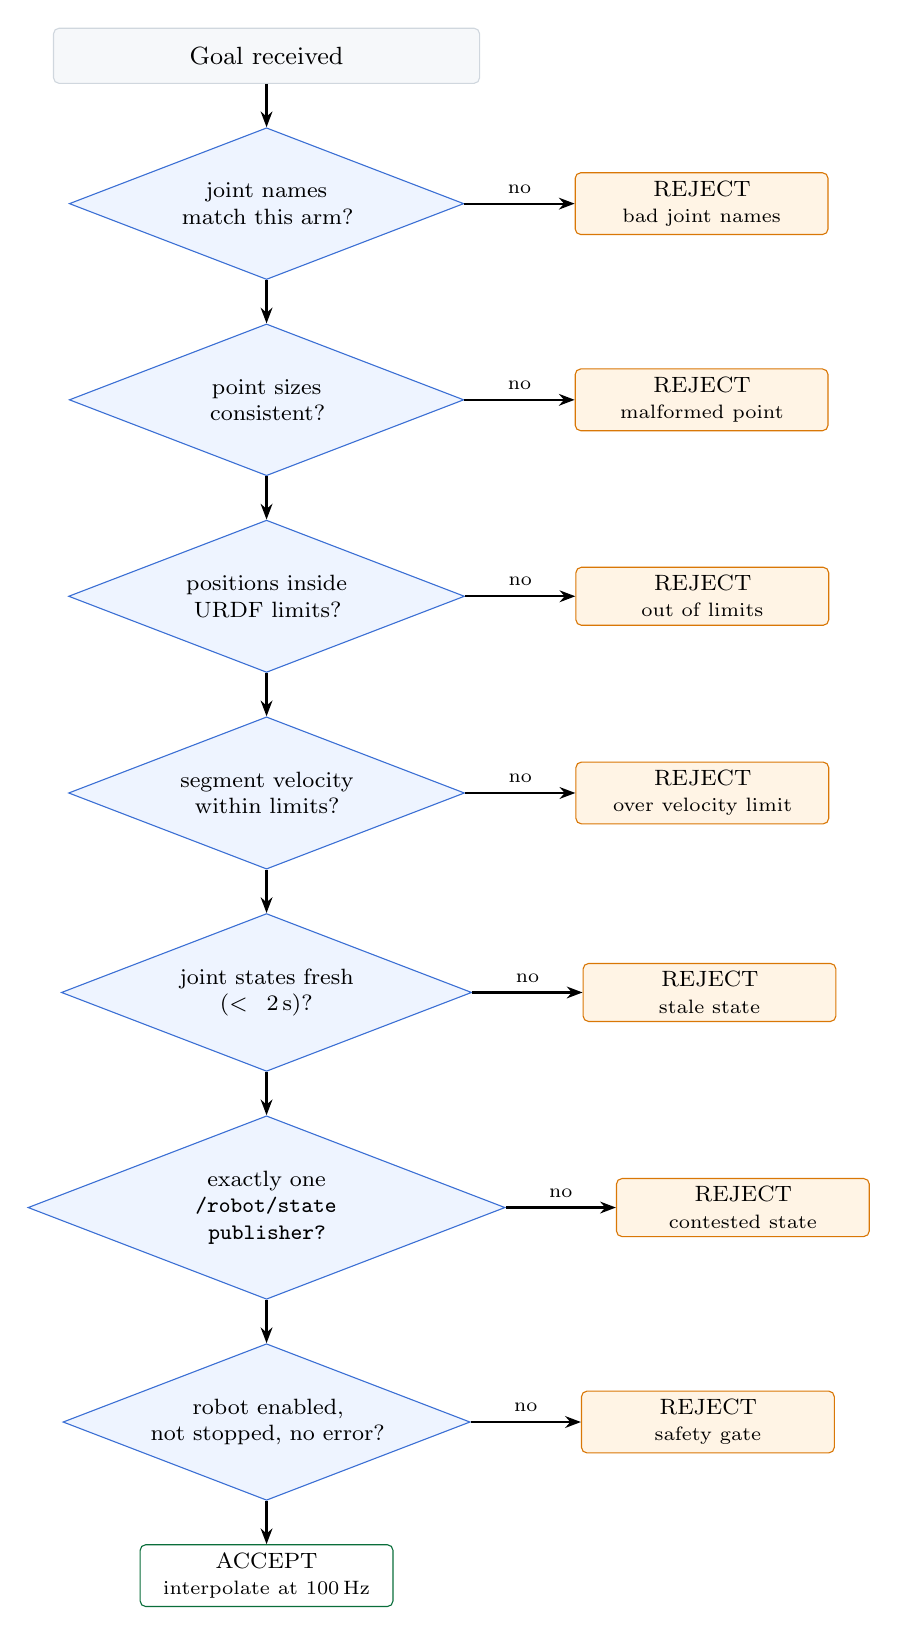
\begin{tikzpicture}[
  font=\small, node distance=5.5mm,
  stepbox/.style={draw, rounded corners=2pt, align=center, text width=52mm,
               minimum height=7mm, inner sep=3pt, fill=codebg, draw=coderule},
  dec/.style={draw, diamond, aspect=2.6, align=center, inner sep=1pt,
              text width=34mm, font=\footnotesize, fill=notebg, draw=noterule},
  bad/.style={draw, rounded corners=2pt, align=center, fill=warnbg,
              draw=warnrule, font=\footnotesize, text width=30mm, inner sep=3pt},
  ok/.style={draw, rounded corners=2pt, align=center, fill=white,
             draw=string, font=\footnotesize, text width=30mm, inner sep=3pt},
  flow/.style={-{Stealth[length=2mm]}, thick},
]

\node[stepbox] (goal) {Goal received};
\node[dec, below=of goal] (names)  {joint names\\match this arm?};
\node[dec, below=of names] (counts) {point sizes\\consistent?};
\node[dec, below=of counts] (limits) {positions inside\\URDF limits?};
\node[dec, below=of limits] (vel) {segment velocity\\within limits?};
\node[dec, below=of vel] (fresh) {joint states fresh\\($<2$\,s)?};
\node[dec, below=of fresh] (state) {exactly one\\\ttfamily/robot/state\\publisher?};
\node[dec, below=of state] (enabled) {robot enabled,\\not stopped, no error?};
\node[ok, below=of enabled] (accept) {ACCEPT\\\scriptsize interpolate at 100\,Hz};

\foreach \a/\b in {goal/names, names/counts, counts/limits, limits/vel,
                   vel/fresh, fresh/state, state/enabled, enabled/accept}
  \draw[flow] (\a) -- (\b);

\node[bad, right=14mm of names]   (r1) {REJECT\\\scriptsize bad joint names};
\node[bad, right=14mm of counts]  (r2) {REJECT\\\scriptsize malformed point};
\node[bad, right=14mm of limits]  (r3) {REJECT\\\scriptsize out of limits};
\node[bad, right=14mm of vel]     (r4) {REJECT\\\scriptsize over velocity limit};
\node[bad, right=14mm of fresh]   (r5) {REJECT\\\scriptsize stale state};
\node[bad, right=14mm of state]   (r6) {REJECT\\\scriptsize contested state};
\node[bad, right=14mm of enabled] (r7) {REJECT\\\scriptsize safety gate};

\foreach \a/\b in {names/r1, counts/r2, limits/r3, vel/r4, fresh/r5,
                   state/r6, enabled/r7}
  \draw[flow] (\a) -- node[font=\scriptsize, above]{no} (\b);

\end{tikzpicture}
}
\caption{What a goal has to pass before the arm moves. The 25 cases in
\texttt{dry\_run\_test} are the executable form of this diagram, and run in CI on
every push.}
\label{fig:gate}
\end{figure}

Once a goal is accepted, the shim interpolates it at 100\,Hz and publishes
position commands for as long as the goal is active. Because
\texttt{joint\_command} has a 0.2\,s timeout, holding a position means continuing
to command it --- so the shim keeps commanding the final point for
\texttt{hold\_duration\_sec} after the trajectory ends rather than falling silent
and letting the arm sag into gravity compensation.

\subsection{Tolerances}

Two checks run during motion, both taken from the values the legacy Rethink
trajectory action server actually shipped enabled
(\texttt{PositionJoint\-Trajectory\-Action\-Server}):

\begin{itemize}
  \item \texttt{path\_tolerance\_rad} (0.2): abort if a joint lags the command
    actually published by more than this. Note \emph{published}, not the raw
    interpolated setpoint --- comparing against a setpoint the shim never sent
    would blame the arm for the shim's own clamping.
  \item \texttt{stopped\_velocity\_tolerance} (0.25): after the final point has
    been held for \texttt{goal\_time\_sec}, abort if a joint is still moving
    faster than this.
\end{itemize}

Both \emph{hold} rather than stop, and they hold the \emph{measured} pose. An arm
lagging its setpoint is not necessarily an unsafe arm --- it may simply be blocked
--- and continuing to command a position it cannot reach would drive it harder
into whatever is blocking it.

\subsection{Distinguishing the failure modes}

\texttt{control\_msgs} has standard codes for tolerance failures
(\texttt{PATH\_TOLERANCE\_VIOLATED} $=-4$, \texttt{GOAL\_TOLERANCE\_VIOLATED}
$=-5$) and the shim uses them. It has no code for "cancelled" or "aborted by
safety gate", so the shim uses distinct negative values ($-100$, $-101$) rather
than leaving them at zero. A client that only reads \texttt{error\_code} must not
be able to mistake a safety abort for success.

\section{The safety gate}

\texttt{baxter\_safety\_check} reads \texttt{/robot/state} and reports whether
motion is permissible. One of its checks is less obvious than the rest: it
requires that \emph{exactly one} node publishes \texttt{/robot/state}.

That rule came from an incident. A mock robot left running from an earlier test
published a cheerful "safe" state alongside the real, disabled robot. A gate that
samples the latest message cannot tell which robot it is reading, and it went
unnoticed for about fifteen minutes. Counting publishers is the fix; the
hardware bringup launch also refuses to start if the mock is running.

\section{What still needs the legacy container}

Almost nothing. Bring-up, the interlock tests, supervised motion, tolerance work,
MoveIt and shutdown all run container-free. The exception is untucking.

Tucked arms sit outside the URDF limit table
(Section~\ref{ch:platform}), so the shim rejects that pose by design --- the same
guard rail that makes the workspace refuse to move while tucked. A container-free
untuck would mean hand-publishing joint commands \emph{outside the safety
envelope}, with collision avoidance suppressed, for a large whole-arm motion.

The honest answer is to keep the legacy tool for that one step. The alternative
--- relaxing the shim's limits behind an explicit opt-in so the untuck runs through
the validated path --- is the better long-term design, but it weakens a guard rail
that has already proved useful, and it must never be the default.

\chapter{Supervised motion and measured limits}
\label{ch:hwmotion}

This chapter reports what the robot actually did. Every number has a date and a
session behind it.

\section{What passed, and when}

\begin{table}[h]
\centering
\small
\begin{tabularx}{\linewidth}{@{}llX@{}}
\toprule
\textbf{Gate} & \textbf{Date} & \textbf{Result} \\
\midrule
Bridge, non-motion & 2026-07-22 & Bridged topics at steady rates; robot state readable. \\
Action shims, interlocks & 2026-07-22 & Every malformed and unsafe goal rejected, zero motion. \\
Supervised motion & 2026-07-24 & Both arms, out and back, worst tracking error 0.0078\,rad. \\
MoveIt execution & 2026-07-24 & Planner success, 31 waypoints, settled 0.0128\,rad from target. \\
Speed characterisation & 2026-07-25 & Path-tolerance ceiling found; see below. \\
MoveIt re-run & 2026-07-25 & Mostly aborted on the left arm; see Section~\ref{sec:moveit-hardware}. \\
\bottomrule
\end{tabularx}
\end{table}

All of it on one robot, supervised. None of it establishes sustained duty,
gripper commands, or behaviour on a second machine.

\section{The speed ceiling}
\label{sec:speed}

The first supervised motion ran at 0.117\,rad/s against a shim clamp of
2.0\,rad/s. That is a factor of seventeen of unused headroom, which means no
tolerance figure in the workspace said anything at all about speed. The
2026-07-25 session escalated deliberately, one step at a time, with the recorder
running.

\begin{table}[h]
\centering
\small
\begin{tabular}{@{}rrrrl@{}}
\toprule
\textbf{Step} & \textbf{offset (rad)} & \textbf{duration (s)} & \textbf{rad/s} & \textbf{peak lag} \\
\midrule
1 & 0.35 & 3.0  & 0.12 & 0.037\,rad \\
2 & 0.35 & 1.5  & 0.23 & 0.094\,rad \\
3 & 0.50 & 1.0  & 0.50 & \textbf{0.198\,rad $\rightarrow$ abort} \\
4 & 0.50 & 0.5  & 1.00 & not reached \\
5 & 0.50 & 0.35 & 1.43 & not reached \\
\bottomrule
\end{tabular}
\end{table}

It stopped at step 3 with \texttt{left\_s1 lags its setpoint by 0.202 rad (limit
0.200)}. The arm then held to 0.0004\,rad over six seconds --- the abort-and-hold
path worked exactly as designed.

\begin{figure}[h]
\centering
% Measured on BR-01, 2026-07-25 (I20). Three points, one straight line, and the
% reason path_tolerance_rad is a speed limit rather than a safety margin.
% Source: docs/hardware_day_plan.md P4a escalation table.
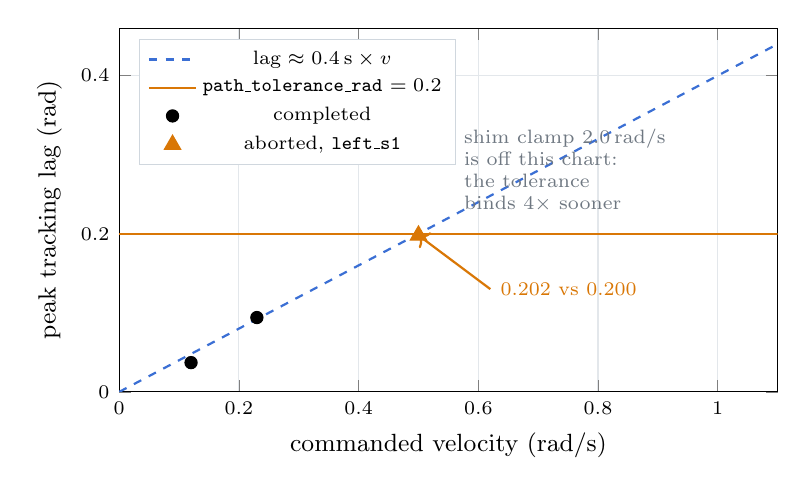
\begin{tikzpicture}
\begin{axis}[
  width=0.82\linewidth, height=6.2cm,
  xlabel={commanded velocity (rad/s)},
  ylabel={peak tracking lag (rad)},
  xmin=0, xmax=1.1, ymin=0, ymax=0.46,
  grid=major, grid style={coderule!60},
  legend pos=north west,
  legend style={font=\scriptsize, draw=coderule},
  label style={font=\small}, tick label style={font=\scriptsize},
]

% lag = 0.4 s * velocity -- the arm runs a constant time behind its setpoint.
\addplot[domain=0:1.1, samples=2, thick, noterule, dashed]
  {0.4*x};
\addlegendentry{$\mathrm{lag} \approx 0.4\,\mathrm{s} \times v$}

% The tolerance that stops the move.
\addplot[domain=0:1.1, samples=2, thick, warnrule]
  {0.2};
\addlegendentry{\texttt{path\_tolerance\_rad} $=0.2$}

\addplot[only marks, mark=*, mark size=2.2pt, black]
  coordinates {(0.12,0.037) (0.23,0.094)};
\addlegendentry{completed}

\addplot[only marks, mark=triangle*, mark size=3.4pt, warnrule]
  coordinates {(0.50,0.198)};
\addlegendentry{aborted, \texttt{left\_s1}}

\node[font=\scriptsize, align=left, anchor=west, text=comment]
  at (axis cs:0.56,0.28) {shim clamp 2.0\,rad/s\\is off this chart:\\the tolerance\\binds 4$\times$ sooner};

\draw[<-, thick, warnrule] (axis cs:0.50,0.198) -- (axis cs:0.62,0.13)
  node[anchor=west, font=\scriptsize, text=warnrule] {0.202 vs 0.200};

\end{axis}
\end{tikzpicture}

\caption{Three measured points and one straight line. Lag is proportional to
commanded velocity, so the path tolerance is a speed limit in disguise.}
\label{fig:lag}
\end{figure}

The three points fall on a line: $\mathrm{lag} \approx 0.4\,\mathrm{s} \times v$.
The arm runs a roughly constant \emph{time} behind its setpoint, which is what a
series-elastic arm under a proportional controller does.

That reframes the tolerance completely. \texttt{path\_tolerance\_rad} $= 0.2$
divided by 0.4\,s gives about 0.5\,rad/s, and that is the practical speed ceiling
of this workspace on this robot. The shim's 2.0\,rad/s per-cycle clamp is
unreachable --- the tolerance binds four times sooner. Anybody reading the clamp
as the speed limit is reading the wrong number.

\begin{notebox}[Two things this does \emph{not} license]
Do not tighten \texttt{path\_tolerance\_rad}: it is the speed limit, not a safety
margin with slack in it. And do not raise it at a desk. Whether 0.3--0.4 is safe
is an open experiment for a supervised session, not a default someone changes in
a config file.
\end{notebox}

A related result from the same session: \texttt{speed\_ratio} had no measurable
effect across 0.1, 0.2 and 0.3. The client's own interpolation is the binding
constraint, so \texttt{duration} is the knob that changes speed.

\section{MoveIt on hardware}
\label{sec:moveit-hardware}

MoveIt planned and executed on the robot on 2026-07-24. The 2026-07-25 re-run,
with eleven goals per arm, went differently:

\begin{table}[h]
\centering
\small
\begin{tabular}{@{}lrrl@{}}
\toprule
\textbf{Arm} & \textbf{Completed} & \textbf{Aborted} & \textbf{Failure} \\
\midrule
Left  & 3 of 11 & 8 & \texttt{PATH\_TOLERANCE\_VIOLATED} on \texttt{left\_w0} / \texttt{left\_e0} \\
Right & 9 of 11 & 2 & --- \\
\bottomrule
\end{tabular}
\end{table}

Both arms were driven by the same \texttt{both\_arms} plans, and every left-arm
abort landed at exactly the tolerance limit on a wrist or elbow joint. The
mechanism is consistent with Section~\ref{sec:speed}: MoveIt plans at default
velocity scaling, the wrist joints permit 4.0\,rad/s against the shoulder's 1.5,
so a time-parameterised plan drives the wrists fastest and they are the first to
exceed a lag budget that corresponds to about 0.5\,rad/s.

\subsection{Workaround}

On this robot, drive MoveIt at \texttt{Velocity Scaling: 0.1} in the
MotionPlanning panel, and plan single-arm groups rather than \texttt{both\_arms}.

\subsection{What is not yet known}

Whether this is an asymmetric \emph{plan} or an asymmetric \emph{arm} is
undecided. A \texttt{both\_arms} plan is not required to distribute motion
symmetrically, so the left arm may simply have drawn the faster half. The
decisive experiment is to command the same joint on each arm --- the
\texttt{joint} parameter of the direct client exists for this --- at matched
speeds, with the recorder running. The recorder was not running during the
MoveIt re-run, which is precisely why the question is still open.

\section{Joint states arrive from two publishers}
\label{sec:jointstate-merge}

\texttt{/robot/joint\_states} is published by two nodes: arm joints from one,
gripper joints from another. A client keeping only the most recent message sees
no arm joints in roughly a third of messages.

The symptom is not a clean error. It looks like intermittent missing data,
timeouts that come and go, and readings that are stale for no visible reason ---
the sort of thing that gets blamed on the network or the robot. Clients on the
hardware path merge positions by name across messages and tolerate an incomplete
view rather than treating it as a fault.

There is a related defect in the bridge worth knowing about before adding topics:
its subscriber negotiates with only the \emph{first} publisher the master lists,
so on a multi-publisher topic it silently receives a subset. Measured effect:
\texttt{/robot/joint\_states} arrives at about 100\,Hz instead of its real
138\,Hz, and gripper joint states never arrive at all.

\chapter{Verification}
\label{ch:verify}

Everything in this chapter runs without a robot.

\section{One command}

\begin{lstlisting}
bash scripts/sim_smoke.sh          # gates + gazebo + moveit
bash scripts/sim_smoke.sh gates    # no Gazebo, no GPU
\end{lstlisting}

It exits zero only if every check passed, and prints its log directory otherwise.
The full run takes about four minutes.

The script asserts \emph{numbers}, not just exit codes. A client can exit zero
having moved the wrong joint, or having printed nothing at all, so every
\texttt{max\_error} is parsed and compared, a minimum count of verified lines is
required, and the exact cancellation log strings must appear.

\begin{notebox}[Teardown is part of the test]
After each launch the script sends one \texttt{SIGINT} and then fails if any
Gazebo, bridge, controller, \texttt{robot\_state\_publisher}, \texttt{move\_group}
or RViz process survives. It never escalates to \texttt{SIGKILL} to make the check
pass --- that would hide precisely the defect being looked for. Leftovers from a
previous run also look identical to a teardown failure in the next one, which is
why the script refuses to start if a simulation is already running.
\end{notebox}

\section{What each gate protects}

\begin{table}[h]
\centering
\small
\begin{tabularx}{\linewidth}{@{}lX@{}}
\toprule
\textbf{Check} & \textbf{The failure it exists to catch} \\
\midrule
Publish hygiene & A placeholder contact address shipping in a release. \\
\texttt{compileall} & Syntax errors in files no test imports. \\
\texttt{ruff --select F} & Unused imports and undefined names. Neither compilation nor import checks notice an unused import; nine of them once survived a refactor because nothing looked. \\
\texttt{colcon test} & The joint-limit selection logic, which is branchy and otherwise only exercised by a full simulation run. \\
\texttt{dry\_run\_test} & All 25 shim safety cases, without a robot. \\
\texttt{check\_urdf} & A model that expands but is not a valid tree. \\
SRDF matrix & The 54-pair collision matrix and the two hand-added pairs, whose loss only manifests on hardware. \\
Cleanup-handler AST guard & A cancel that raises inside \texttt{except BaseException} and replaces the exception \texttt{main()} dispatches on, turning Ctrl-C into a misleading error. \\
\bottomrule
\end{tabularx}
\end{table}

\section{What stays manual}

The RViz MotionPlanning panel. It has to actually load: no
\texttt{Exception caught while processing action 'loadRobotModel'}, a populated
planner dropdown rather than \texttt{NO PLANNING LIBRARY LOADED}, a 6-DOF
interactive marker on each gripper, and no \texttt{No robot state or robot model
loaded}. Automating that costs more than it catches; a person looking at the
panel for ten seconds is the cheaper check.

\begin{safetybox}[If all four symptoms appear at once]
Check your locale. Qt calls \texttt{setlocale(LC\_ALL, "")} before
\texttt{rclcpp::init}, so under a comma-decimal locale rcl parses every double
parameter as a string and \texttt{loadRobotModel} dies. The MoveIt launch pins
\texttt{LC\_NUMERIC=C} for the RViz node; if you launch RViz another way, set it
yourself.
\end{safetybox}

\section{Continuous integration}

CI runs the hardware-free set on every push: publish hygiene, build,
compile/import, the cleanup-handler guard, \texttt{ruff}, the unit tests, the
dry run, URDF expansion, and the static MoveIt and controller-config checks. It
installs no ROS~1, no robot-network tooling, and no Zenoh.

It deliberately does not run Gazebo. A full simulation needs a GUI-capable runner
and is slow and flaky in CI; the manual smoke and \texttt{sim\_smoke.sh} cover it
locally, and local teardown remains a required gate before any release.


\appendix
\chapter{Command sheet}
\label{app:commands}

Condensed from \texttt{docs/sim\_test\_commands.md}, which is the maintained
version. Nothing here needs a robot.

\section{Build}

\begin{lstlisting}
conda deactivate                       # if any env is active
which python3                          # want /usr/bin/python3
rm -rf build install log
source /opt/ros/jazzy/setup.bash
colcon build --base-paths src --symlink-install --packages-skip baxter_bridge
source install/setup.bash
\end{lstlisting}

\section{Hardware-free gates}

\begin{lstlisting}
bash scripts/sim_smoke.sh gates
\end{lstlisting}

Or individually:

\begin{lstlisting}
grep -RIn '@example\.com' src --include='package.xml' SECURITY.md CODE_OF_CONDUCT.md
python3 -m compileall -q src/baxter_bringup src/baxter_gz_sim \
    src/baxter_moveit_config src/baxter_examples src/baxter_hardware_bridge
ruff check --select F src scripts --exclude src/baxter_common_ros2
colcon test --base-paths src --packages-select baxter_examples
colcon test-result --verbose
ros2 run baxter_hardware_bridge dry_run_test          # OVERALL: PASS, 25 cases
ros2 run xacro xacro src/baxter_gz_sim/urdf/baxter_gz_control.urdf.xacro > /tmp/b.urdf
check_urdf /tmp/b.urdf
\end{lstlisting}

\texttt{ruff} is not a ROS package and \texttt{rosdep} will not install it:
\texttt{pipx install ruff}.

\section{Gazebo}

Terminal 1:

\begin{lstlisting}
ros2 launch baxter_gz_sim sim_rviz.launch.py headless:=false
\end{lstlisting}

Terminal 2:

\begin{lstlisting}
ros2 control list_controllers                          # 3 active
ros2 topic echo /joint_states --once                   # 17 joints
ros2 launch baxter_examples sim_tiny_trajectory.launch.py
ros2 run baxter_examples sim_tiny_trajectory --ros-args \
    -p use_sim_time:=true -p joint:=e1
ros2 run baxter_examples sim_tiny_trajectory --ros-args \
    -p use_sim_time:=true -p cancel_after_sec:=1.0
\end{lstlisting}

\section{MoveIt}

Terminal 1 (stop the previous launch first):

\begin{lstlisting}
ros2 launch baxter_moveit_config sim_moveit_rviz.launch.py headless:=false
\end{lstlisting}

Terminal 2:

\begin{lstlisting}
ros2 action list                                       # /move_action
ros2 run baxter_examples moveit_left_tiny
ros2 run baxter_examples moveit_tiny --ros-args -p group:=right_arm
ros2 run baxter_examples moveit_tiny --ros-args -p group:=both_arms
ros2 run baxter_examples moveit_pose --ros-args -p group:=left_arm -p delta_z:=0.05
ros2 run baxter_examples ik_service_client --ros-args -p limb:=left
ros2 run baxter_examples ik_service_client --ros-args -p limb:=left -p x:=9.0
ros2 run baxter_examples moveit_tiny --ros-args -p cancel_after_sec:=1.0
\end{lstlisting}

The unreachable IK query must exit non-zero.

\section{Teardown}

One Ctrl+C per launch, then:

\begin{lstlisting}
pgrep -a -f 'gz sim|ros_gz_bridge|move_group|rviz2|robot_state_publisher|ros2_control_node'
\end{lstlisting}

No output is the pass. Gazebo exiting $-2$ is expected; a surviving process is a
gate failure.

\section{Expected output tokens}

\begin{table}[h]
\centering
\small
\begin{tabularx}{\linewidth}{@{}lX@{}}
\toprule
\textbf{Check} & \textbf{Expected} \\
\midrule
Publish hygiene & no output \\
Dry run & \texttt{OVERALL: PASS}, 25 cases \\
Unit tests & \texttt{16 tests, 0 errors, 0 failures} \\
SRDF & \texttt{acm\_pairs=54} \\
Motion & \texttt{max\_error} $\le 0.02$\,rad, every arm and direction \\
Direct cancel & \texttt{Controller goal canceled; holding position} \\
MoveIt cancel & \texttt{MoveGroup goal canceled; holding position} \\
Unreachable IK & \texttt{INVALID POSE}, exit 1 \\
\bottomrule
\end{tabularx}
\end{table}

\chapter{Reference tables}
\label{app:tables}

\section{Joint limits}

Transcribed from \texttt{baxter\_description/urdf/baxter\_base/baxter\_base.urdf.xacro}.
Left and right carry identical limits, so one table serves both arms. Prefix with
\texttt{left\_} or \texttt{right\_}.

\begin{table}[h]
\centering
\small
\begin{tabular}{@{}llrrr@{}}
\toprule
\textbf{Suffix} & \textbf{Segment} & \textbf{Lower (rad)} & \textbf{Upper (rad)} & \textbf{Max vel (rad/s)} \\
\midrule
\texttt{s0} & shoulder roll   & $-1.70167993878$ & $1.70167993878$ & 1.5 \\
\texttt{s1} & shoulder pitch  & $-2.147$         & $1.047$         & 1.5 \\
\texttt{e0} & upper-arm roll  & $-3.05417993878$ & $3.05417993878$ & 1.5 \\
\texttt{e1} & elbow pitch     & $-0.05$          & $2.618$         & 1.5 \\
\texttt{w0} & wrist roll      & $-3.059$         & $3.059$         & 4.0 \\
\texttt{w1} & wrist pitch     & $-1.57079632679$ & $2.094$         & 4.0 \\
\texttt{w2} & wrist roll      & $-3.059$         & $3.059$         & 4.0 \\
\bottomrule
\end{tabular}
\end{table}

The parked pose puts \texttt{s1} at approximately $-2.175$\,rad, outside this
table. That is expected and is why the shim refuses to move a tucked robot.

\section{Shim parameters}

\begin{table}[h]
\centering
\small
\begin{tabularx}{\linewidth}{@{}llX@{}}
\toprule
\textbf{Parameter} & \textbf{Default} & \textbf{Meaning} \\
\midrule
\texttt{side} & \texttt{left} & Which arm this instance serves. \\
\texttt{mock\_mode} & \texttt{false} & Validate without publishing commands. \\
\texttt{speed\_ratio} & 0.1 & Legacy scaling. Measured to have no effect; \texttt{duration} is the binding constraint. \\
\texttt{command\_rate} & 100.0\,Hz & Interpolation and publish rate. \\
\texttt{command\_timeout} & 0.2\,s & Robot-side timeout; commands must keep arriving. \\
\texttt{max\_step\_rad\_per\_cycle} & 0.02 & Per-cycle clamp, i.e. 2.0\,rad/s. Unreachable in practice --- see below. \\
\texttt{hold\_duration\_sec} & 1.0\,s & How long the final point keeps being commanded. \\
\texttt{joint\_states\_stale\_sec} & 2.0\,s & Reject goals if state is older than this. \\
\texttt{path\_tolerance\_rad} & 0.2 & Abort if a joint lags the published command by more than this. \\
\texttt{stopped\_velocity\_tolerance} & 0.25 & Abort if still moving after the settle window. \\
\texttt{goal\_time\_sec} & 0.1\,s & Settle window before the stopped-velocity check. \\
\bottomrule
\end{tabularx}
\end{table}

\begin{notebox}
\texttt{max\_step\_rad\_per\_cycle} looks like the speed limit and is not. At
0.4\,s of lag per rad/s of commanded velocity, \texttt{path\_tolerance\_rad}
$= 0.2$ aborts at about 0.5\,rad/s --- four times below the clamp. See
Section~\ref{sec:speed}.
\end{notebox}

\section{Result codes}

\begin{table}[h]
\centering
\small
\begin{tabularx}{\linewidth}{@{}rlX@{}}
\toprule
\textbf{Code} & \textbf{Name} & \textbf{Meaning} \\
\midrule
$0$    & \texttt{SUCCESSFUL} & Goal completed and verified. \\
$-4$   & \texttt{PATH\_TOLERANCE\_VIOLATED} & A joint lagged too far during motion. Arm holds. \\
$-5$   & \texttt{GOAL\_TOLERANCE\_VIOLATED} & Still moving after the settle window. Arm holds. \\
$-10$  & \texttt{START\_STATE\_IN\_COLLISION} & From \texttt{move\_group}; see the SRDF section. \\
$-31$  & \texttt{NO\_IK\_SOLUTION} & Unreachable pose. \\
$-100$ & (local) canceled & Cancelled by the client. Not a standard code. \\
$-101$ & (local) aborted & Rejected or aborted by the safety gate. Not a standard code. \\
\bottomrule
\end{tabularx}
\end{table}

\section{Topics and actions}

\begin{table}[h]
\centering
\small
\begin{tabularx}{\linewidth}{@{}llX@{}}
\toprule
\textbf{Name} & \textbf{Side} & \textbf{Role} \\
\midrule
\texttt{/joint\_states} & sim & 17 joints from the broadcaster. \\
\texttt{/left\_arm\_controller/follow\_joint\_trajectory} & sim & Arm action. \\
\texttt{/right\_arm\_controller/follow\_joint\_trajectory} & sim & Arm action. \\
\texttt{/move\_action} & both & MoveIt planning and execution. \\
\texttt{/robot/joint\_states} & hardware & Bridged. Two publishers; merge by name. \\
\texttt{/robot/ref\_joint\_states} & hardware & Robot's own reference, $\approx$140\,Hz. \\
\texttt{/robot/state} & hardware & \texttt{AssemblyState}; exactly one publisher required. \\
\texttt{/robot/limb/*/joint\_command} & hardware & Position commands out. \\
\texttt{/robot/limb/*/follow\_joint\_trajectory} & hardware & Shim actions. \\
\bottomrule
\end{tabularx}
\end{table}

\section{Measured values}

\begin{table}[h]
\centering
\small
\begin{tabularx}{\linewidth}{@{}llX@{}}
\toprule
\textbf{Quantity} & \textbf{Value} & \textbf{Source} \\
\midrule
Sim goal tolerance & 0.02\,rad & Controller config; every client checks it. \\
Best hardware tracking error & 0.0078\,rad & 2026-07-24, 0.117\,rad/s. \\
MoveIt hardware settling & 0.0128\,rad & 2026-07-24, 31 waypoints. \\
Lag coefficient & $\approx 0.4$\,s $\times v$ & 2026-07-25, three points. \\
Practical speed ceiling & $\approx 0.5$\,rad/s & 2026-07-25, at tolerance 0.2. \\
\texttt{/robot/joint\_states} rate & 138\,Hz & 2026-07-24 (bridge sees $\approx$100). \\
\texttt{/robot/ref\_joint\_states} rate & 140\,Hz & 2026-07-24. \\
SRDF collision pairs & 54 & Checked in CI. \\
Dry-run cases & 25 & Checked in CI. \\
\bottomrule
\end{tabularx}
\end{table}


\end{document}
